\documentclass[12pt]{article}
\usepackage{amsmath,geometry,times,bm,float}
\geometry{margin=1.00in}
\floatplacement{figure}{H}

\title{Math 297 Project II}
\author{Jiaqi Liu}\date{6 March 2022}
\usepackage{Sweave}
\begin{document}\maketitle\thispagestyle{empty}
\Sconcordance{concordance:Project2.tex:Project2.Rnw:%
1 7 1 1 0 1 1 1 15 3 1 1 7 3 1 1 2 1 0 1 1 1 3 5 0 1 2 1 9 3 1 1 16 15 %
0 1 2 4 1 1 14 16 0 1 2 1 1 1 2 1 0 4 1 1 18 20 0 1 2 2 1 1 2 1 0 2 1 1 %
21 23 0 1 2 1 1 1 2 1 0 2 1 1 18 20 0 1 2 4 1 1 31 30 0 1 2 5 1 3 0 1 2 %
9 1 1 7 1 1 1 2 1 0 1 15 14 0 1 2 5 0 1 4 11 1 1 2 1 0 1 13 12 0 1 2 6 %
0 1 5 17 1 1 2 1 0 1 1 1 12 11 0 1 2 5 0 1 4 17 1 1 2 1 0 1 1 1 11 10 0 %
1 2 4 0 1 2 61 1 1 2 1 0 3 1 8 0 1 7 7 1}


\section{Parametric bootstrap}
We have $n=973$ observations on two variables $X$ and $Y$. In Project I, we used regressogram, linear spline, kernel and lowess to fit the data. In this section, we use Efron's procedure to find the best regression model.  Just like what we did in Project I, we first consider a linear spline model with a very large number of knots $k_{big}=n/\log n$. This model will give us the estimated residual variance $\widehat{\sigma}^2$ and serve as the big model for the bootstrap.

Let $\{\widehat{y}_i^{big}, i=1,...,n\}$ be the estimated value under this big elspline model with $k_{big}$ number of bins. We obtain $\widehat\sigma^2 = 0.991894464747625$ and $\{\widehat{y}^{big}_i, i=1,...,n\}$. 


With the help of $\widehat{\sigma}^2$ and $\widehat{y}^{big}$, we are going to generate $B=100$ psuedo data set. To be more precise, for every pair $(x_i,y_i)$, we generate a large number $B$ of simulated observations according to the approximated normal distribution $N(\widehat{y}^{big}_i,\widehat\sigma^2)$. On each pseudo data set, we are going to estimate risks for each models. We use the $n\times B$ matrix to record the pseudo data set denoted as $(x_i, y_i^{*p})$ for $i=1,...n$ and $p=1,...,B$.
\begin{Schunk}
\begin{Sinput}
> B = 100
> pseudo = matrix(0, nrow = n, ncol = B)
> for (i in 1:B){
+   pseudo[,i] = yhat_big + rnorm(n, 0, sigmahat)
+ }
\end{Sinput}
\end{Schunk}
For each pseudo data set $(x_i, y_i^{*p})_{i=1}^{n}$, we will apply Efron's procedure to estimate risks. This requires us to generate $B=100$ simulated observations $(x_i, y_i^{*p,b})$ for $i=1,...n$ and $b=1,...,B$ according to the parametric bootstrap $N(\widehat{y}_i^{*p, big}, \widehat{sigma}^2)$. Here $(\widehat{y}_i^{*p,big})_{i=1}^{n}$ is the fitted value for the pseudo data under the big model and $\widehat{\sigma}$ is the estimated variance as before. We first calculate $(\widehat{y}_i^{*p,big})_{i=1}^{n}$.

Next, we estimate risks for each model. Using the results in Project I, we consider the regressogram with 42 number of bins, linear spline model with 5 number of knots, kernel model with bandwidth 0.25, and lowess model with bandwidth 0.25. Risks are estimated using Efron's procedure.

\subsection{Estimated risk for regressogram with 42 number of bins}
\begin{Schunk}
\begin{Sinput}
> regressores <- function(x, y, nbins){
+   xy <- data.frame(x=x, y=y)
+   xy <- xy[order(xy$x),]
+   z <- cut(xy$x,breaks=seq(min(xy$x),max(xy$x),length=round(nbins)+1),
+            labels=1:round(nbins),include.lowest=TRUE)
+   xyz <- data.frame(xy,z=z)
+   MEANS <- c(by(xyz$y,xyz$z,FUN=mean))
+   new = split(xyz, xyz$z)
+   ans = rep(0, times = n+1)
+   ans[1:n] = MEANS[z]
+   for (i in 1:round(nbins)){
+     ans[n+1] = ans[n+1] + sum((new[[i]][["y"]]-MEANS[i])^2)
+   }
+   return(ans)
+ }
> k1 = 42
> Errhat_reg = rep(0, times = B)
> covhat_reg = rep(0, times = B)
> boot = matrix(0, nrow = n, ncol = B)
> meanboot = rep(0, times = n)
> for (i in 1:B){
+   err_reg = regressores(xx, pseudo[,i], k1)[n+1]
+   for (j in 1:B){
+     boot[,j] = pseudo_hat[,i] + rnorm(n, 0, sigmahat)
+   }
+   for (j in 1:n){
+     meanboot[j]= mean(boot[j,])
+   }
+   for (j in 1:B){
+     muhatstar = regressores(xx, boot[,j], k1)[1:n]
+     covhat_reg[j] = sum(muhatstar*(boot[,j]-meanboot))/(B-1)
+   }
+   Errhat_reg[i] = err_reg + 2*sum(covhat_reg)
+ }
\end{Sinput}
\end{Schunk}

\subsection{Estimated risk for linear spline model with 5 number of knots}
\begin{Schunk}
\begin{Sinput}
> k2 = 5
> knots = seq(min(xx) ,max(xx), length=k2+2)
> knots = knots[2:k2+1]
> Errhat_sp = rep(0, times = B)
> covhat_sp = rep(0, times = B)
> for (i in 1:B){
+   pseudo_dat = data.frame(x=xx, y=pseudo[,i])
+   spmodel = lm(y ~ lspline(xx, knots), data=pseudo_dat)
+   err_sp = sum(resid(spmodel)^2)
+   for (j in 1:B){
+     boot[,j] = pseudo_hat[,i] + rnorm(n, 0, sigmahat)
+   }
+   for (j in 1:n){
+     meanboot[j]= mean(boot[j,])
+   }
+   for (j in 1:B){
+     newdat = data.frame(x=xx, y=boot[,j])
+     spmodel_new = lm(y ~ lspline(x,knots), data=newdat)
+     muhatstar = fitted(spmodel_new)
+     covhat_sp[j] = sum(muhatstar*(boot[,j]-meanboot))/(B-1)
+   }
+   Errhat_sp[i] = err_sp + 2*sum(covhat_sp)
+ }
\end{Sinput}
\end{Schunk}


\subsection{Estimated risk for kernel model with bandwidth 0.25}
\begin{Schunk}
\begin{Sinput}
> k3 = 0.25
> Errhat_ker = rep(0, times = B)
> covhat_ker = rep(0, times = B)
> for (i in 1:B){
+   pseudo_dat = data.frame(x=xx, y=pseudo[,i])
+   sort_pseudo_dat = pseudo_dat[order(pseudo_dat$x),]
+   knmodel = ksmooth(sort_pseudo_dat$x, sort_pseudo_dat$y, 'normal', bandwidth = k3, x.points=sort_pseudo_dat$x)
+   yhat_ker = knmodel$y
+   err_ker = sum((yhat_ker-sort_pseudo_dat$y)^2)
+   for (j in 1:B){
+     boot[,j] = pseudo_hat[,i] + rnorm(n, 0, sigmahat)
+   }
+   for (j in 1:n){
+     meanboot[j]= mean(boot[j,])
+   }
+   for (j in 1:B){
+     newdat = data.frame(x=xx, y=boot[,j], z=meanboot)
+     sortnewdat = newdat[order(newdat$x),]
+     knmodelnew = ksmooth(sortnewdat$x, sortnewdat$y, 'normal', bandwidth = k3, x.points=sortnewdat$x)
+     muhatstar = knmodelnew$y
+     covhat_ker[j] = sum(muhatstar*(sortnewdat$y-sortnewdat$z))/(B-1)
+   }
+   Errhat_ker[i] = err_ker + 2*sum(covhat_ker)
+ }
\end{Sinput}
\end{Schunk}

\subsection{Estimated risk for lowess model with bandwidth 0.25}
\begin{Schunk}
\begin{Sinput}
> k4 = 0.25
> Errhat_low = rep(0, times = B)
> covhat_low = rep(0, times = B)
> for (i in 1:B){
+   pseudo_dat = data.frame(x=xx, y=pseudo[,i])
+   lowessmd = loess(y~x, pseudo_dat, span = k4)
+   err_low = sum(lowessmd$residuals^2)
+   for (j in 1:B){
+     boot[,j] = pseudo_hat[,i] + rnorm(n, 0, sigmahat)
+   }
+   for (j in 1:n){
+     meanboot[j]= mean(boot[j,])
+   }
+   for (j in 1:B){
+     newdat = data.frame(x=xx, y=boot[,j])
+     lowessmd_new = loess(y~x, newdat, span = k4)
+     muhatstar = fitted(lowessmd_new)
+     covhat_low[j] = sum(muhatstar*(boot[,j]-meanboot))/(B-1)
+ }
+   Errhat_low[i] = err_low + 2*sum(covhat_low)
+ }
\end{Sinput}
\end{Schunk}

\subsection{Hypothesis testing}
With four sequences of risk estimates under each model, we are going to use the hypothesis testing to diagonose the best model.The idea is as follows. Suppose we have two models A and B, and their corresponding sequences of estimates risks $(Err^A_{p})_{p=1}^{B}$ and $(Err^B_{p})_{p=1}^{B}$. Then the risk differences between model A and B will be the sequence $(Diff^{A,B})_{p=1}^{B}=(Err^A_{p}-Err^B_{p})_{p=1}^{B}$. The null hypothesis is model A is no better than B and model B is no better than B, i.e. $H_0: Err^A=Err^B$. For every $\alpha\in (0,1)$, we can find values $a$ and $b$ such that $(1-\alpha)B$ of the estimated risk differences stay in the interval $[a,b]$. Then $[a,b]$ will be our $(1-alpha)*100\%$ confidence interval. According to the duality between the confidence interval and the hypothesis testing, the largest $\alpha$ for which $[a,b]$ contains 0 will be the p value for our hypothesis testing. If the p value is very small, we reject the null hypothesis and have good reason to believe that either model A is better than model B or model B is better than model A.  If the confidence interval falls in the positive real line, we conclude that model B is better than model A while if the confidence interval falls in the negative real line, we conclude that model A is better than model B.

We first write a function which has inputs riskA, riskB and threshold, and outputs the better model by calculating p values. Specifically, under certain threshold, output 0 means that the null hypothesis was not rejected, 1 means model A is better and 2 means model B is better.
\begin{Schunk}
\begin{Sinput}
> hypotest_p <- function(riskA, riskB, threshold){
+   diff = riskA - riskB
+   diff = sort(diff)
+   if (diff[1]>0){
+     return(2)
+   }
+   if (diff[B]<0){
+     return(1)
+   }
+   i = 1
+   j = B
+   while (diff[i+1] < 0){
+     i = i + 1
+   }
+   while (diff[j-1] > 0){
+     j = j - 1
+   }
+   alpha1 = 2*i/B
+   alpha2 = 1 - 2*j/B
+   alpha = min(alpha1,alpha2)
+   if (alpha > threshold){
+     return(0)
+   }
+   if (B - j > i){
+     return(2)
+   }
+   if (B - j < i){
+     return(1)
+   }
+ }
> p_reg_sp = hypotest_p(Errhat_reg, Errhat_sp, 0.1)
> p_reg_ker = hypotest_p(Errhat_reg, Errhat_ker, 0.1)
> p_reg_low = hypotest_p(Errhat_reg, Errhat_low, 0.1)
> p_sp_ker = hypotest_p(Errhat_sp, Errhat_ker, 0.1)
> p_sp_low = hypotest_p(Errhat_sp, Errhat_low, 0.1)
> p_ker_low = hypotest_p(Errhat_ker, Errhat_low, 0.1)
\end{Sinput}
\end{Schunk}
Therefore, according to the hypothesis testing, at the level of $5\%$, Regressogram is better than all the other three models, linear spline model and lowess are better than kernel regression, and linear spline model is no better than lowess model and lowess model is no better than linear spline model. Therefore, we have good reasons to believe that the regressogram with 42 number of bins is the best regression model. We draw the graph of the regressogram with 42 number of bins below.
\begin{figure}
\begin{center}
\caption{Regressogram with 42 number of bins is the best model}
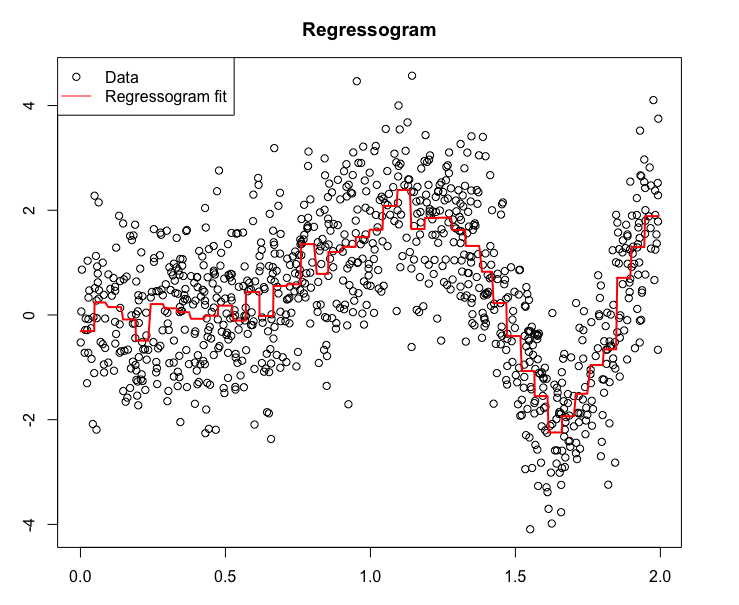
\includegraphics[scale=0.50]{optimal regressogram}
\end{center}
\end{figure}

\section{Cross Validation}
In this section, we apply 7-fold cross-validation on each models -- regressograms, linear splines, kernel regression and lowess, to estimate the optimal smoothing parameters. We use ``Caret" package to random sample data poitns and create folds.

\subsection{Regressogram}
\begin{Schunk}
\begin{Sinput}
> predict_err_reg = rep(0, times = 100)
> for (j in 1:100){
+   predict_err = rep(0, times = 7)
+   for (i in 1:7){
+     validat = dat[flds[[i]], ]
+     traindat = dat[-flds[[i]],]
+     xy = data.frame(x = traindat$xx, y = traindat$yy)
+     xy = xy[order(xy$x),]
+     z = cut(xy$x,breaks=seq(min(dat$xx),max(dat$xx),length=j+1),labels=1:j,include.lowest=TRUE)
+     xyz = data.frame(xy,z=z)
+     MEANS = c(by(xyz$y,xyz$z,FUN=mean))
+     vali_z = cut(validat$xx,breaks=seq(min(dat$xx),max(dat$xx),length=j+1),labels=1:j,include.lowest=TRUE)
+     predict_err[i] = sum((MEANS[vali_z]-validat$yy)^2)/7
+   }
+   predict_err_reg[j] = sum(predict_err)
+ }
> optimal_nbins = which.min(predict_err_reg)
> #par(mar = c(3, 3, 3, 3)) 
> #plot(1:100, predict_err_reg,pch=16,xlab = "Number of bins", ylab = "Predicted error")
\end{Sinput}
\end{Schunk}

The optimal number of bins is $42$, which is the same as the one obtained in Project I. Furthermore, the graph of the predicted errors for regressograms with different number of bins has the same trend as the graph of the estimated risks of the regressograms with different number of bins plotted in Project I.
\begin{figure}
\begin{center}
\caption{Predicted error for regressogram with different number of bins}
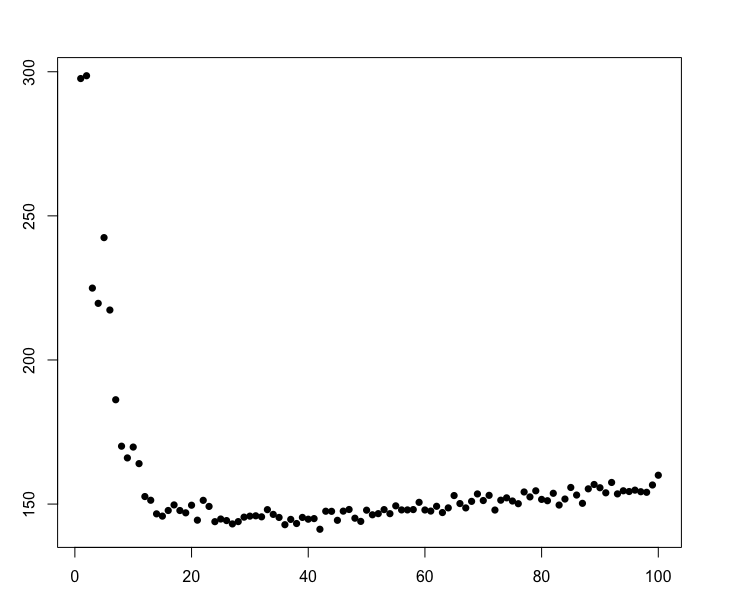
\includegraphics[scale=0.50]{regressogram find the optimal}
\end{center}
\end{figure}
The fitted curve of the regressogram with the optimal number of bins is as in Figure 1.


\subsection{Linear spline model}
\begin{Schunk}
\begin{Sinput}
> predict_err_sp = rep(0, times = 20)
> for (j in 1:20){
+   predict_err = rep(0, times = 7)
+   for (i in 1:7){
+     validat = dat[flds[[i]], ]
+     traindat = dat[-flds[[i]],]
+     knots = seq(min(xx), max(xx), length = j+2)
+     knots = knots[2:j+1]
+     spmodel = lm(yy ~ lspline(xx, knots), data = traindat)
+     vali_pred = predict(spmodel, newdata = validat) 
+     predict_err[i] = sum((vali_pred - validat$yy)^2)/7
+   }
+   predict_err_sp[j] = sum(predict_err)
+ }
> optimal_knot = which.min(predict_err_sp)
> 
> #par(mar = c(3, 3, 3, 3)) 
> #plot(1:20, predict_err_sp,pch=16, xlab = "Number of knots", ylab = "Predicted error")
\end{Sinput}
\end{Schunk}
The optimal number of knots is $10$, which is different from the one obtained using Efron's procedure. However, if we plot the predicted errors for linear spline models with different number of knots, we can see that the predicted error at 5 and 10 are similar. This might indicate that if we choose a different random sampling in the cross validation fold, there is a chance that the optimal number of knots may be 5. Furthermore, if we compare this graph with the plot of the estimated errors of the linear spline models with different number of knots plotted in Project I, they have the same trend.
\begin{figure}
\begin{center}
\caption{Predicted error for linear spline models with different number of knots}
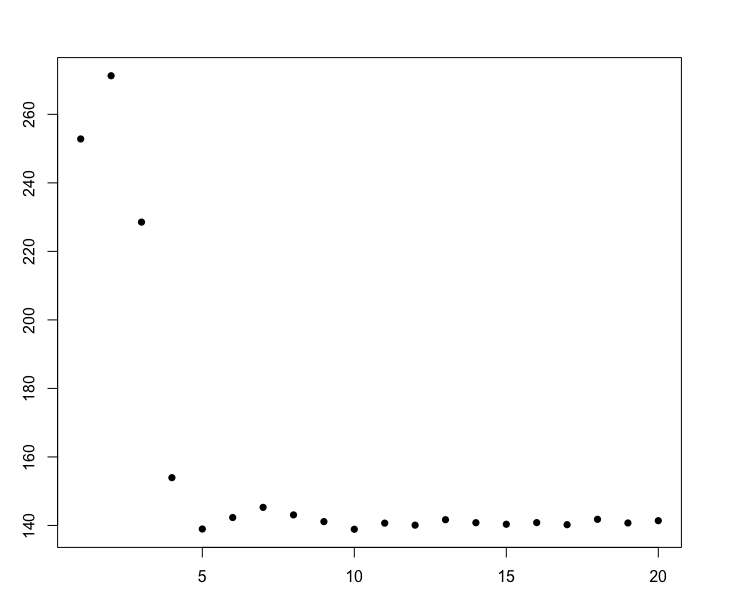
\includegraphics[scale=0.50]{linear spline find the optimal knot}
\end{center}
\end{figure}
The fitted curve of the linear spline model with the optimal number of knots is as follows.
\begin{figure}
\begin{center}
\caption{Optimal linear spline model}
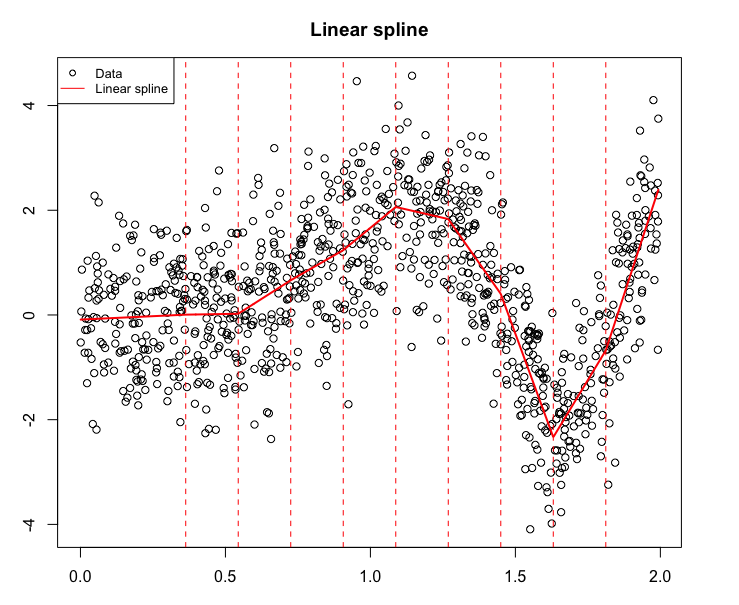
\includegraphics[scale=0.50]{linear spline}
\end{center}
\end{figure}



\subsection{Kernel regression}
\begin{Schunk}
\begin{Sinput}
> predict_err_ker = rep(0, times = 20)
> h = seq(from = 0.05, to = 1, length.out = 20)
> for (j in 1:20){
+   predict_err = rep(0, times = 7)
+   for (i in 1:7){
+     validat = dat[flds[[i]], ]
+     sort_validat = validat[order(validat$xx),]
+     traindat = dat[-flds[[i]],]
+     sort_traindat = traindat[order(traindat$xx),]
+     knmodel = ksmooth(sort_traindat$xx, sort_traindat$yy, 'normal', bandwidth = h[j], x.points=sort_validat$xx)
+     predict_err[i] = sum((knmodel$y - sort_validat$yy)^2)/7
+   }
+   predict_err_ker[j] = sum(predict_err)
+ }
> optimal_ker = h[which.min(predict_err_ker)]
> #par(mar = c(3, 3, 3, 3)) 
> #plot(h, predict_err_ker,pch=16,xlab = "Bandwidth", ylab = "Predicted error")
\end{Sinput}
\end{Schunk}
The optimal bandwidth is $0.1$. If we plot the predicted error for kernel regression with different bandwidths, we see that there isn't a big difference between the prediction errors for 0.1 and 0.15.
\begin{figure}
\begin{center}
\caption{Predicted error for kernel regression with different bandwidths}
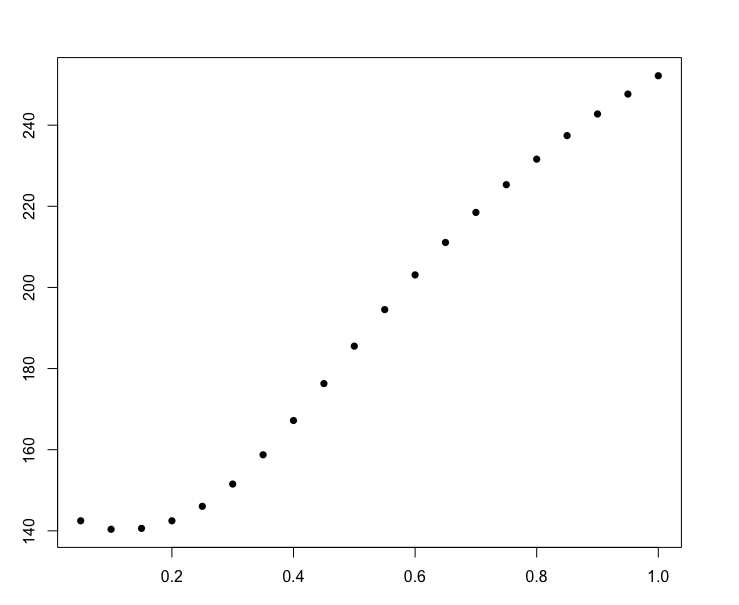
\includegraphics[scale=0.50]{kernel find the optimal bandwidth}
\end{center}
\end{figure}

If we look at the graph for the kernel regression with 0.1 bandwidth, it is a littlbe bit over fit. The optimal bandwidth using Efron's procedure is 0.25, which is better compared with the one obtained using cross validation.
\begin{figure}
\begin{center}
\caption{Optimal kernel regression}
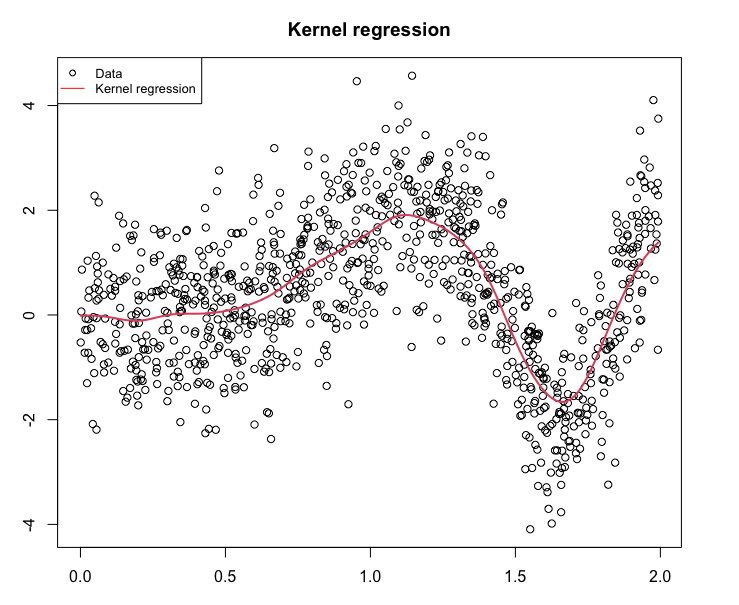
\includegraphics[scale=0.50]{kernel regression}
\end{center}
\end{figure}


\subsection{Lowess model}
\begin{Schunk}
\begin{Sinput}
> predict_err_low = rep(0, times = 30)
> h = seq(from = 0.05, to = 0.95, length.out = 30)
> for (j in 1:30){
+   predict_err = rep(0, times = 7)
+   for (i in 1:7){
+     validat = dat[flds[[i]], ]
+     traindat = dat[-flds[[i]],]
+     lowessmd = loess(yy~xx, traindat, span = h[j], control=loess.control(surface="direct"))
+     vali_pred = predict(lowessmd, newdata = validat)
+     predict_err[i] = sum((vali_pred - validat$yy)^2)/7
+   }
+   predict_err_low[j] = sum(predict_err)
+ }
> # In the lowess regression funciton ``loess", we add ``control=loess.control(surface="direct")" to avoid NA returns in prediction.
> optimal_span = h[which.min(predict_err_low)]
\end{Sinput}
\end{Schunk}
The optimal span is $0.267241379310345$, which is similar to the optimal span 0.25 we obtained using Efron's procedure. The plot for predicted errors of lowess model with different spans and the fitted curve for the optimal lowess model are as follows.
\begin{figure}
\begin{center}
\caption{Predicted error for lowess models with spans}
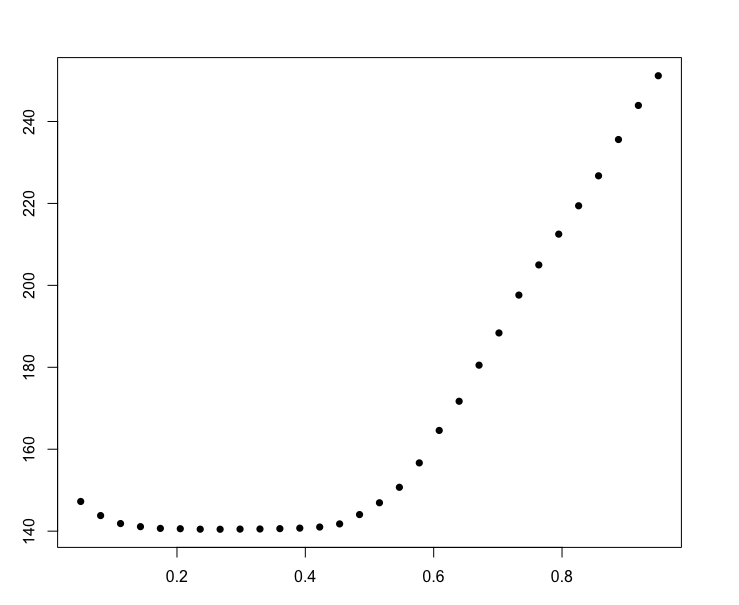
\includegraphics[scale=0.5]{find optimal span lowess}
\end{center}
\end{figure}
\begin{figure}
\begin{center}
\caption{Optimal lowess model}
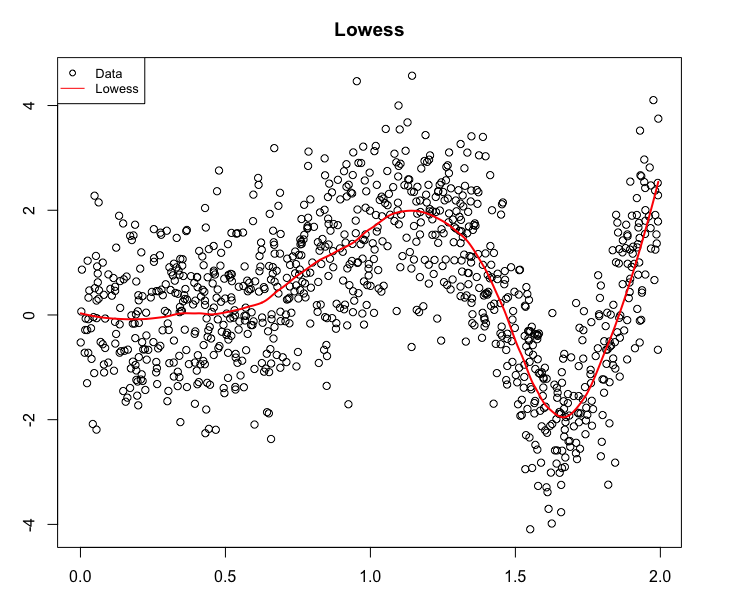
\includegraphics[scale=0.5]{lowess}
\end{center}
\end{figure}

\section{Summary}
A Gaussian process (GP) is a stochastic process (a collection of random variables indexed by time or space), such that every finite collection of those random variables has a multivariate normal distributionFrom the function-space (or equivalently, the weight-space view), we can view the Gaussian process as a distribution over functions, and Gaussian process regression model as the inference conducted in the space of functions. Using this connection, if we project the inputs into a high-dimensional feature space, then we can apply the Bayesian treatment of the linear model in this feature space. It was shown in Section 2.1 and 2.2 that these two point of views will reach identical regression results. In this summary, we will show how the Gaussian process regression model is derived under the view of function-space.

Consider a data set of $n$ observations, $(\mathbf{x}_i, y_i)_{i=1}^{n}$, where $\mathbf{x}$ is an input vector of dimension $D$ and $y$ is a scalar output. First of all, a Gaussian process is completely determined by its mean function and covariance function. Therefore, it suffices to estimate the mean function and the covariance function
\[
m(\mathbf{x})=E[f(\mathbf{x})], \qquad k(c)=E\left[(f(\mathbf{x}_p)-m(\mathbf{x}_p))(f(\mathbf{x}_q)-m(\mathbf{x}_q))\right].
\]
Modeling with noisy observations $y=f(\mathbf{x}+\epsilon)$ where $\epsilon$ is the Gaussian noise with variance $\sigma_n^2$, we consider the squared exponential covariance function of the form
\[
\text{cov}(y_p,y_q)=k(\mathbf{x}_p,\mathbf{x}_q)+\sigma_n^2\delta_{pq} = \exp\left(-\frac{1}{2}\left|\mathbf{x}_p-\mathbf{x}_q\right|^2\right)+\sigma_n^2I.
\]
Let $\mathbf{y}$ be the target values, the above equation can be written as
\[
\text{cov}(\mathbf{y})=K(X,X)+\sigma^2 I.
\]
Define $\mathbf{f}_*$ to be the function values at the test locations under the prior, then the joint distribution between $\mathbf{y}$ and $\mathbf{f}_*$ is
\[
\begin{pmatrix}
\mathbf{y} \\
\mathbf{f}_*
\end{pmatrix}\sim N\left(\begin{pmatrix}
\mathbf{0} \\
\mathbf{0}
\end{pmatrix},\begin{pmatrix}
K(X,X)+\sigma_n^2I &K(X,X_*)\\
K(X_*,X) & K(X_*,X_*)
\end{pmatrix}\right).
\]
Since the conditional distribution for normal distributions is still normal distribution, the prediction equation for the Gaussian process regression model is
\[
\mathbf{f}_*|X,\mathbf{y}, X_*\sim N(\bar{\mathbf{f}}_*, cov(\mathbf{f}_*)),
\]
where 
\[
\bar{\mathbf{f}}_*=E[\mathbf{f}_*|X,\mathbf{y},X_*]=K(X_*,X)[K(X,X)+\sigma_n^2I]^{-1}\mathbf{y},
\]
\[
\text{cov}=K(X_*,X_*)-K(X_*,X)\left[K(X,X)+\sigma_n^2I\right]^{-1}K(X,X_*).
\]
Furthermore, the marginal likelihood $p(\mathbf{y}|X)$ can be computed explicitly
\[
\log p(\mathbf{y}|X)=\log \int p(\mathbf{y}|\mathbf{f},X)p(\mathbf{f}|X)d\mathbf{f}=-\frac{1}{2}\mathbf{y}^T(K+\sigma_n^2I)^{-1}\mathbf{y}-\frac{1}{2}\log|K+\sigma_n^2I|-\frac{n}{2}\log 2\pi.
\]
In practicise, the large inverse matrix $(K(X,X)+\sigma_n^2I)^{-1}$ can be computed using the Cholesky decomposition.


\section{Gaussian process regression model}
In this section, we are going to use ``GauPro" package to fit a Gaussian process regression model. We plot the fitted curve estimate in red and the 95\% credible intervals in blue. 
\begin{Schunk}
\begin{Sinput}
> library(GauPro)
> x = dat$xx
> y = dat$yy
> gp = GauPro(x, y, parallel = FALSE)
> #plot(dat, main = 'Gaussian process regression', xlab = 'x', ylab = 'y')
> #curve(gp$predict(x), add=T, col='red',lwd=2)
> #curve(gp$predict(x)+1.96*gp$predict(x, se=T)$se, add=T, col='blue', lwd=2,lty='dashed')
> #curve(gp$predict(x)-1.96*gp$predict(x, se=T)$se, add=T, col='blue', lwd=2,lty='dashed')
> #legend("topleft", legend=c("Fitted curve", "Boundaries of credible interval"), col=c("red", "blue"),lty =c(1, 2), cex=0.8)
\end{Sinput}
\end{Schunk}
We see that the Gaussian process regression wroks well and most of data points are within the $95\%$ credible interval.
\begin{figure}
\begin{center}
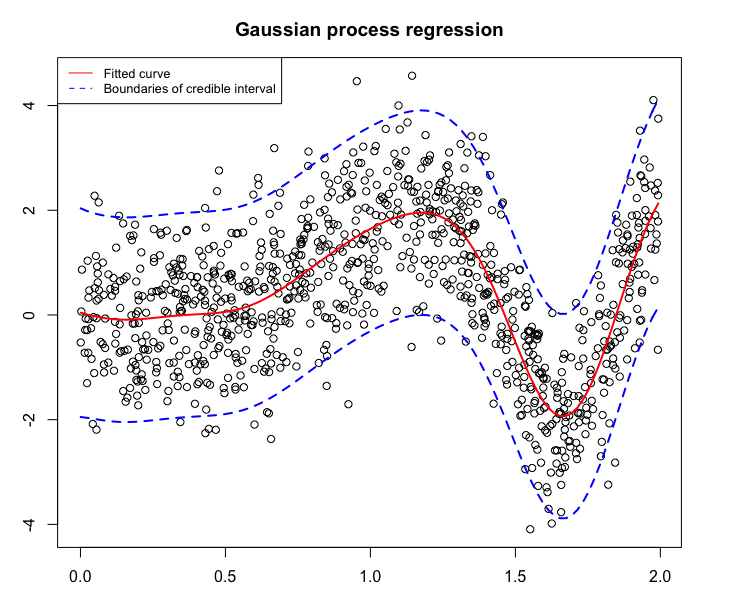
\includegraphics[scale=0.50]{Gaussian process regression}
\end{center}
\end{figure}

\end{document}
